\documentclass{article}
\usepackage[utf8]{inputenc}
\usepackage{amsmath}

\usepackage{tikz}
\usetikzlibrary{bayesnet}

\title{figuretest}
\author{ }
\date{June 2017}

\begin{document}

\maketitle

\section{Introduction}


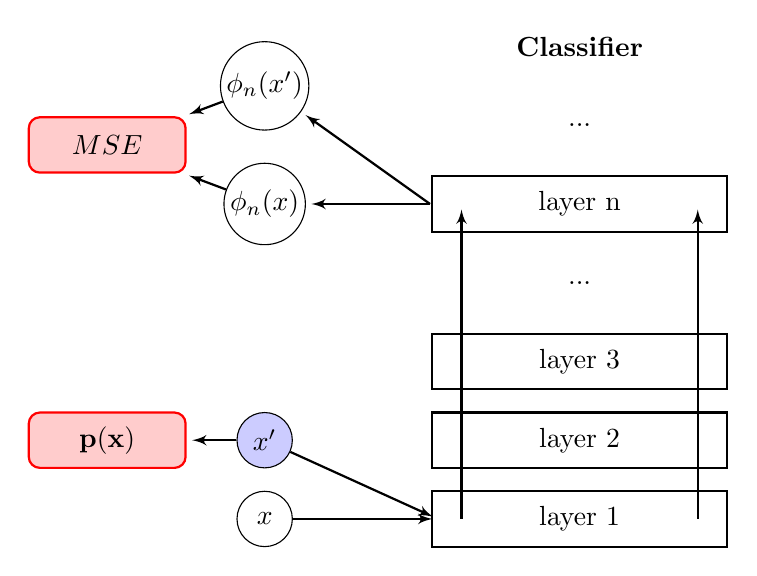
\begin{tikzpicture}
[auto,
 net/.style ={rectangle, draw=blue, thick, fill=blue!20, text width=3em,align=center, rounded corners, minimum height=2em},
 loss/.style ={rectangle, draw=red, thick, fill=red!20, text width=5em,align=center, rounded corners, minimum height=2em},
 klloss/.style ={rectangle, draw=red, thick, fill=red!20, text width=13em,align=center, rounded corners, minimum height=2em},
 dist/.style ={rectangle, draw=black, thick, text width=5em,align=center, rounded corners, minimum height=2em},
 layer/.style ={rectangle, draw=black, thick, text width=10em,align=center, minimum height=2em},
 line/.style ={draw, thick, -latex',shorten >=2pt},
 cloud/.style ={draw=red, thick, ellipse,fill=red!20,
 minimum height=1em}]
\draw (-4, 0) node[latent] (x) {$x$};
\draw (-4, 1) node[latent, fill=blue!20] (x') {$x'$};
\draw (0, 0) node[layer] (l1) {layer 1};
\draw (0, 1) node[layer] (l2) {layer 2};
\draw (0, 2) node[layer] (l3) {layer 3};
\draw (0, 3) node[] (dot) {...};
\draw (0, 4) node[layer] (ln) {layer n};
\draw (0, 5) node[] (dot2) {...};
\draw (0, 6) node[] (name) {\textbf{Classifier}};
\draw (-4, 4) node[latent] (fx) {$\phi_n (x)$};
\draw (-4, 5.5) node[latent] (fx') {$\phi_n (x')$};
\draw (-6, 1) node[loss] (px) {$\mathbf{p(x)}$};
\draw (-6, 4.75) node[loss] (mse) {$MSE$};
\draw[line] (x) -- (-1.8, 0);
\draw[line] (x') -- (-1.8, 0);
\draw[line] (-1.9, 4) -- (fx);
\draw[line] (-1.9, 4) -- (fx');
\draw[line] (fx) -- (mse);
\draw[line] (fx') -- (mse);
\draw[line] (x') -- (px);
\draw[line] (-1.5, 0) -- (-1.5, 4);
\draw[line] (1.5, 0) -- (1.5, 4);
\end{tikzpicture}
\\ ~ \\

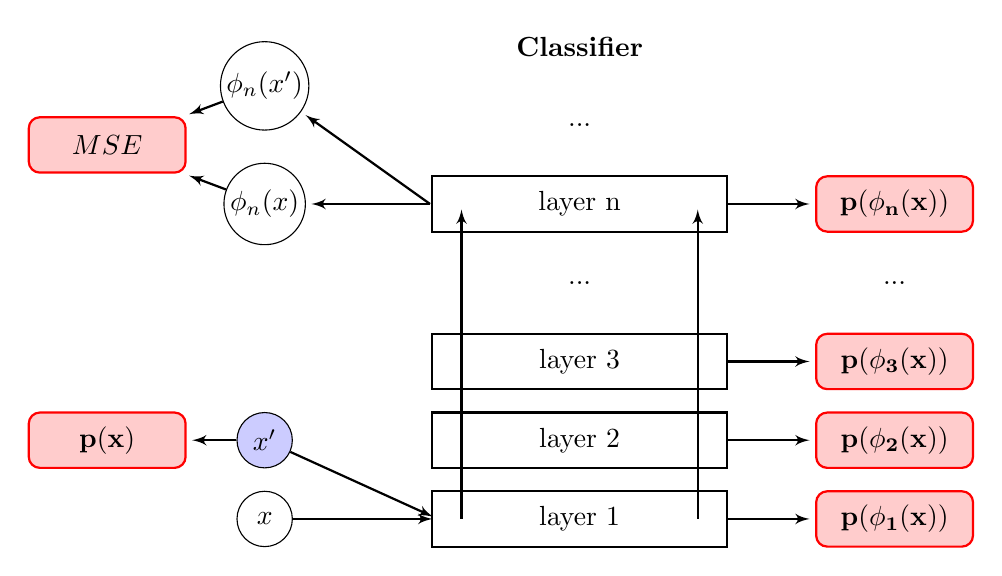
\begin{tikzpicture}
[auto,
net/.style ={rectangle, draw=blue, thick, fill=blue!20, text width=3em,align=center, rounded corners, minimum height=2em},
loss/.style ={rectangle, draw=red, thick, fill=red!20, text width=5em,align=center, rounded corners, minimum height=2em},
klloss/.style ={rectangle, draw=red, thick, fill=red!20, text width=13em,align=center, rounded corners, minimum height=2em},
dist/.style ={rectangle, draw=black, thick, text width=5em,align=center, rounded corners, minimum height=2em},
layer/.style ={rectangle, draw=black, thick, text width=10em,align=center, minimum height=2em},
line/.style ={draw, thick, -latex',shorten >=2pt},
cloud/.style ={draw=red, thick, ellipse,fill=red!20,
	minimum height=1em}]
\draw (-4, 0) node[latent] (x) {$x$};
\draw (-4, 1) node[latent, fill=blue!20] (x') {$x'$};
\draw (0, 0) node[layer] (l1) {layer 1};
\draw (0, 1) node[layer] (l2) {layer 2};
\draw (0, 2) node[layer] (l3) {layer 3};
\draw (0, 3) node[] (dot) {...};
\draw (0, 4) node[layer] (ln) {layer n};
\draw (0, 5) node[] (dot2) {...};
\draw (0, 6) node[] (name) {\textbf{Classifier}};
\draw (-4, 4) node[latent] (fx) {$\phi_n (x)$};
\draw (-4, 5.5) node[latent] (fx') {$\phi_n (x')$};
\draw (-6, 1) node[loss] (px) {$\mathbf{p(x)}$};
\draw (-6, 4.75) node[loss] (mse) {$MSE$};
\draw (4, 0) node[loss] (pfx1) {$\mathbf{p(\phi_1(x))}$};
\draw (4, 1) node[loss] (pfx2) {$\mathbf{p(\phi_2(x))}$};
\draw (4, 2) node[loss] (pfx3) {$\mathbf{p(\phi_3(x))}$};
\draw (4, 3) node[] (dot3) {...};
\draw (4, 4) node[loss] (pfxn) {$\mathbf{p(\phi_n(x))}$};
\draw[line] (x) -- (-1.8, 0);
\draw[line] (x') -- (-1.8, 0);
\draw[line] (-1.9, 4) -- (fx);
\draw[line] (-1.9, 4) -- (fx');
\draw[line] (fx) -- (mse);
\draw[line] (fx') -- (mse);
\draw[line] (x') -- (px);
\draw[line] (-1.5, 0) -- (-1.5, 4);
\draw[line] (1.5, 0) -- (1.5, 4);
\draw[line] (l1) -- (pfx1);
\draw[line] (l2) -- (pfx2);
\draw[line] (l3) -- (pfx3);
\draw[line] (ln) -- (pfxn);
\end{tikzpicture}
\\ ~ \\

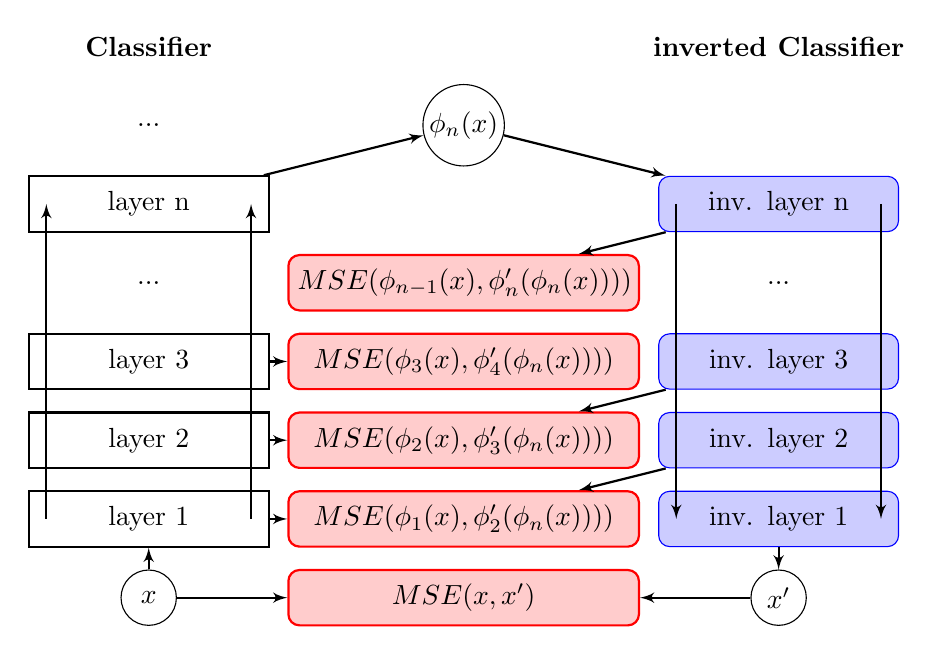
\begin{tikzpicture}
[auto,
net/.style ={rectangle, draw=blue, fill=blue!20, text width=3em,align=center, rounded corners, text width=8em, minimum height=2em},
loss/.style ={rectangle, draw=red, thick, fill=red!20, text width=12em,align=center, rounded corners, minimum height=2em},
klloss/.style ={rectangle, draw=red, thick, fill=red!20, text width=13em,align=center, rounded corners, minimum height=2em},
dist/.style ={rectangle, draw=black, thick, text width=5em,align=center, rounded corners, minimum height=2em},
layer/.style ={rectangle, draw=black, thick, text width=8em,align=center, minimum height=2em},
line/.style ={draw, thick, -latex'},
cloud/.style ={draw=red, thick, ellipse,fill=red!20,
	minimum height=1em}]
\draw (0, -1) node[latent] (x) {$x$};
\draw (8, -1) node[latent] (x') {$x'$};
\draw (0, 0) node[layer] (l1) {layer 1};
\draw (0, 1) node[layer] (l2) {layer 2};
\draw (0, 2) node[layer] (l3) {layer 3};
\draw (0, 3) node[] (dot) {...};
\draw (0, 4) node[layer] (ln) {layer n};
\draw (0, 5) node[] (dot2) {...};
\draw (0, 6) node[] (name) {\textbf{Classifier}};
\draw (8, 0) node[net] (l1') {inv. layer 1};
\draw (8, 1) node[net] (l2') {inv. layer 2};
\draw (8, 2) node[net] (l3') {inv. layer 3};
\draw (8, 3) node[] (dot3) {...};
\draw (8, 4) node[net] (ln') {inv. layer n};
\draw (8, 6) node[] (name) {\textbf{inverted Classifier}};
\draw (4, 5) node[latent] (fx) {$\phi_n (x)$};
\draw (4, -1) node[loss] (msex) {$MSE(x, x')$};
\draw (4, 0) node[loss] (msefx1) {$MSE(\phi_1(x), \phi_2'(\phi_n(x))))$};
\draw (4, 1) node[loss] (msefx2) {$MSE(\phi_2(x), \phi_3'(\phi_n(x))))$};
\draw (4, 2) node[loss] (msefx3) {$MSE(\phi_3(x), \phi_4'(\phi_n(x))))$};
\draw (4, 3) node[loss] (msefxn) {$MSE(\phi_{n-1}(x), \phi_n'(\phi_n(x))))$};
\draw[line] (-1.3, 0) -- (-1.3, 4);
\draw[line] (1.3, 0) -- (1.3, 4);
\draw[line] (6.7, 4) -- (6.7, 0);
\draw[line] (9.3, 4) -- (9.3, 0);
\draw[line] (ln) -- (fx);
\draw[line] (fx) -- (ln');
\draw[line] (x) -- (msex);
\draw[line] (x') -- (msex);
\draw[line] (l2') -- (msefx1);
\draw[line] (l1) -- (msefx1);
\draw[line] (l3') -- (msefx2);
\draw[line] (l2) -- (msefx2);
\draw[line] (l3) -- (msefx3);
\draw[line] (ln') -- (msefxn);
\draw[line] (x) -- (l1);
\draw[line] (l1') -- (x');
\end{tikzpicture}

\end{document}